\newpage
\begin{section}{Power supply from track}

    \begin{subsection}{Theory}
        The transmitter is powered from the train which is powered by the track.
        Drawing power from the train is an easy solution for source of power.
        The power drawn carries a binary signal, by frequency modulating a square wave (squave).
        This squave is a ±18V signal that gives power and instructions to the train, but for our purposes, 
        we only need to extract the power from it.

        \begin{figure}[htbp]
            \centering
            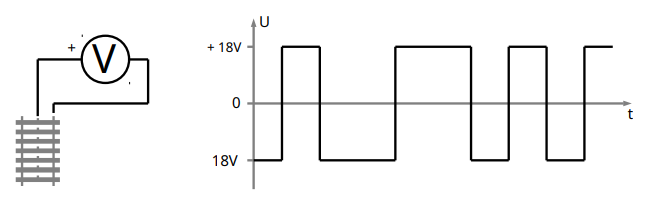
\includegraphics[width=0.8\textwidth]{./figures/src/TrackPower.png}
            \caption{The squave signal and power location on track.}
        \end{figure}

    \end{subsection}
    \begin{subsection}{Implementation}
        With the use of a fullbridge rectifier with capacitor filtering, and a buck converter 
        we convert the AC signal from the squave into a stable positive DC voltage suitable for powering the transmitter.
        \\
        The implementation involves connecting the fullbridge rectifier to the track power input of the train.
        The rectifier converts the AC squave signal into a DC voltage, which is then fed into a buck converter.
        The buck converter steps down the voltage to a level suitable for the transmitter, while also
        ensuring a stable DC output, minimizing ripple and noise that could affect the transmitter's performance.

    \end{subsection}
    \begin{subsection}{Results}

    \end{subsection}
    \begin{subsection}{Discussion}

    \end{subsection}

\end{section}